%% =====================================================================
%% A Leakage-Corrected Reassessment of Metadata Fusion on LIAR
%% IEEEtran journal article (compile with pdfLaTeX + BibTeX).
%% Figures expected under ./figures/.
%% =====================================================================

\documentclass[journal]{IEEEtran}

\usepackage{cite}
\usepackage{amsmath,amssymb,amsfonts}
\usepackage{graphicx}
\usepackage{textcomp}
\usepackage{xcolor}
\usepackage{booktabs}
\usepackage{url}
\usepackage{hyperref}
\hypersetup{hidelinks}

\begin{document}

\title{A Leakage-Corrected Reassessment of Metadata Fusion for Six-Class Political Disinformation Detection on the LIAR Benchmark}

\author{%
  Daniyar~Koishin,%
  \IEEEmembership{ MSc~Student,~Astana~IT~University}%
  \\%
  \textit{Supervisor:}~Tamara~Zhukabayeva,~PhD,~Professor%
  % \thanks{D.~Koishin is with the Department of Computer Science and Engineering, Astana IT University, Astana, Kazakhstan (e-mail: dandevko@gmail.com).}%
}

% \markboth{IEEE Access Submission, April~2026}{Koishin: Leakage-Corrected Metadata Fusion on LIAR}

\maketitle

% ----------------------------------------------------------------------
\begin{abstract}
The LIAR six-class disinformation benchmark has been widely used to argue that hybrid models combining a text encoder with a speaker-credibility metadata branch substantially outperform text-only baselines. We replicate this finding and then audit the credibility-history features used by the standard pipeline. We show that the five-number credibility vector released with LIAR \emph{includes the rating of the current statement itself}, so a hybrid model conditioned on this vector at training and inference time has direct access to the label it is asked to predict. After correcting this leakage---by subtracting the current statement's contribution from each speaker's running counts---the apparent advantage of metadata fusion disappears. We train matched systems on identical splits: three TF-IDF baselines (Naive Bayes, Linear SVM, Random Forest), a text-only fine-tuned roberta-base classifier, and metadata-augmented hybrids in both leaky and leakage-corrected variants. With three independent seeds (42, 1337, 2024), the leaky hybrid attains test macro-F1 of $0.436 \pm 0.004$ (accuracy $0.420 \pm 0.003$), reproducing the published metadata-fusion numbers. The leakage-corrected hybrid drops to $0.284 \pm 0.003$ macro-F1 ($0.284 \pm 0.010$ accuracy), statistically indistinguishable from the text-only RoBERTa baseline ($0.285 \pm 0.007$ macro-F1) and from a matched architectural ablation that masks the metadata branch ($0.287 \pm 0.009$). Per-class analysis confirms that the apparent lift on the extreme classes (\emph{pants-fire}, \emph{mostly-true}) is concentrated entirely in the leaky setting and vanishes once the current rating is held out. We conclude that the published LIAR metadata-fusion gains are substantially attributable to a label-leakage artifact in the credibility-history features, and we recommend that future LIAR work either correct this leakage at preprocessing time or report results in both regimes. All code, configuration files, multi-seed metric JSONs, and per-example prediction artifacts are available at \url{https://github.com/nihsioK/nlp-disinformation-detection-aitu}.
\end{abstract}

\begin{IEEEkeywords}
Disinformation detection, fake news, LIAR dataset, label leakage, RoBERTa, metadata fusion, hybrid models, reproducibility, natural language processing.
\end{IEEEkeywords}

% ======================================================================
\section{Introduction}
\label{sec:introduction}
% ======================================================================
\IEEEPARstart{D}{isinformation} on social platforms is one of the most widely studied problems at the intersection of natural language processing (NLP) and computational social science. Recent surveys estimate that a substantial fraction of online content encountered by average users during election cycles is either misleading or outright false, with measurable downstream effects on public opinion, financial markets, and public-health behaviour~\cite{shu2017,oshikawa2020}. Automated detection systems are therefore of direct practical value, but the fine-grained nature of the task---distinguishing \emph{outright lies} from \emph{exaggerations} and from \emph{mostly-true} statements---makes it fundamentally harder than the binary spam-filtering tasks that dominated earlier text-classification work.

The LIAR benchmark introduced by Wang~\cite{wang2017liar} is the most widely used testbed for fine-grained English political fact-checking. LIAR contains 12{,}836 short statements extracted from PolitiFact, each labelled on a six-point truthfulness scale (\emph{pants-fire}, \emph{false}, \emph{barely-true}, \emph{half-true}, \emph{mostly-true}, \emph{true}) together with 13 metadata fields describing the speaker, the speaker's job and party affiliation, the statement's subject, and a five-number credibility history counting the speaker's ratings in each of the lower five categories. Wang's original CNN classifier obtained 27.4\% test accuracy on the six-class task~\cite{wang2017liar}, and a recurring finding in subsequent work~\cite{shu2017,oshikawa2020,raza2025,papageorgiou2025} is that fusing the text encoder with the credibility-history vector and other speaker metadata raises macro-F1 by 10--15 absolute points over text-only baselines. A recent line of graph- and attention-based models~\cite{zhang2024heterosgt,gu2024,tong2025,zhang2024phd} has built on this premise to design increasingly elaborate multimodal architectures.

This paper revisits that premise. Motivated by the size of the reported metadata-fusion gain---which is large compared with the gain from upgrading the text backbone alone~\cite{devlin2019bert,raza2025}---we re-examined the construction of the credibility-history vector that is shipped with the canonical LIAR release. Counting the speaker's prior \emph{pants-fire}, \emph{false}, \emph{barely-true}, \emph{half-true}, and \emph{mostly-true} ratings is conceptually a leave-one-out operation: when the model is asked to classify a particular statement, the credibility totals available to it should not include the current statement's own rating. In the released schema, however, each statement's credibility-history vector reflects the speaker's full PolitiFact record \emph{at the time the dataset was assembled}, including the statement under classification. The current label therefore leaks into the input through these counts, and a hybrid classifier can learn to read it off.

Our contribution is to quantify the consequences of this leakage on the LIAR six-class task and to provide a matched leakage-corrected baseline for future work:

\begin{itemize}
  \item We implement four model families on an identical preprocessing pipeline, data split, multi-seed evaluation protocol, and ordinal cross-entropy loss: three classical baselines over shared TF-IDF features (Naive Bayes, Linear SVM, Random Forest), a fine-tuned \texttt{roberta-base} text-only classifier, a metadata-augmented hybrid that uses the credibility-history vector \emph{as released} (\emph{leaky} regime, matching prior work), and the same hybrid with leakage corrected by subtracting the current statement's contribution from each speaker's running counts.
  \item We replicate the previously-reported metadata-fusion gain in the leaky regime: averaged over three seeds (42, 1337, 2024), the leaky hybrid attains $0.436 \pm 0.004$ macro-F1 and $0.420 \pm 0.003$ accuracy, broadly consistent with published numbers around 0.41--0.44 macro-F1.
  \item We show that the gain disappears almost entirely once the credibility-history counts are computed in a leakage-free manner. The leakage-corrected hybrid attains $0.284 \pm 0.003$ macro-F1 ($0.284 \pm 0.010$ accuracy), which is statistically indistinguishable from a text-only \texttt{roberta-base} classifier ($0.285 \pm 0.007$) and from a matched ablation that masks the metadata branch entirely ($0.287 \pm 0.009$).
  \item We provide a per-class decomposition that localises the leakage signal. The disproportionate lift on \emph{pants-fire} and \emph{mostly-true} that has been used in the literature as evidence that metadata fusion encodes speaker reputation is observed only in the leaky regime; in the corrected regime the per-class profile of the hybrid model collapses onto the text-only baseline.
\end{itemize}

The remainder of the paper follows the standard IMRAD structure. Section~\ref{sec:related} situates the work in the LIAR and fake-news-detection literature. Section~\ref{sec:method} describes the dataset, preprocessing, four model families, the leaky and leakage-corrected variants of the credibility-history features, and the fusion design. Section~\ref{sec:setup} specifies the experimental setup, including the ordinal loss, hyperparameters, multi-seed protocol, and hardware. Section~\ref{sec:results} reports test-set numbers, per-class analysis, confusion matrices, and the leaky-versus-corrected comparison. Section~\ref{sec:discussion} interprets the findings, connects them to the published literature, and lists the limitations that follow from the fixed LIAR split. Section~\ref{sec:conclusion} closes with future work.

% ======================================================================
\section{Related Work}
\label{sec:related}
% ======================================================================

\subsection{From Classical Machine Learning to Transformers}
Early disinformation-detection systems relied on bag-of-words and TF-IDF features combined with linear classifiers or decision-tree ensembles~\cite{khanam2021,irawan2025,sanahmed2023}. These systems remain attractive because they are inexpensive to train, inspectable, and surprisingly competitive on tasks where lexical cues are strongly correlated with the label. On LIAR in particular, the original CNN of Wang~\cite{wang2017liar} and the linear models reproduced by Rashkin \emph{et~al.}~\cite{shu2017} land within a narrow band around 0.22--0.28 accuracy for the six-class formulation, suggesting that surface lexical features alone provide only a weak signal. Salve~\cite{salve2025} reaches a similar conclusion in a recent Master's thesis comparing TF-IDF pipelines on fact-checking data.

The release of BERT~\cite{devlin2019bert} and its descendants shifted the state of the art across short-text classification, and LIAR-style benchmarks are no exception. Raza \emph{et~al.}~\cite{raza2025} and Papageorgiou \emph{et~al.}~\cite{papageorgiou2025} report 1--3 accuracy-point improvements by replacing TF-IDF features with fine-tuned transformer encoders while keeping the rest of the pipeline fixed. Recurrent and convolutional hybrids~\cite{mahara2022,gundapu2021} explore a middle ground, but none of these text-only systems closes a large fraction of the gap to the human ceiling, which motivates the next wave of work on \emph{augmented} architectures.

\subsection{Metadata and Context-Aware Hybrid Models}
A recurring finding across surveys of the field~\cite{shu2017,oshikawa2020,mahara2022,villela2023} is that the most robust gains come from fusing text with auxiliary context. Su~\cite{su2022} demonstrates that user-network embeddings can increase F1 by up to 29.3\% in a Twitter setting by injecting information about who shares what, and with whom. Hu \emph{et~al.}~\cite{hu2025} and Cao \emph{et~al.}~\cite{cao2025capsule} report the corresponding result at the statement level: combining textual content with credibility-style user features is especially useful when historically credible users exhibit semantic anomalies, a failure mode that a text-only classifier cannot detect by construction. Kuntur \emph{et~al.}~\cite{kuntur2024} generalise the observation to out-of-distribution settings, arguing that metadata fusion is one of the few mechanisms by which detectors generalise across topical shifts. Murayama \emph{et~al.}~\cite{murayama2021} and Papanastasiou~\cite{papanastasiou2020} model the same intuition at a different level of abstraction, treating propagation and speaker reputation as temporal priors rather than features.

On LIAR specifically, the closest reference points to ours are the hybrid LSTM with attention proposed by Long \emph{et~al.}~\cite{long2017fakenews}, which reached 0.415 macro-F1 by conditioning an LSTM classifier on the speaker-profile attributes, and more recent graph-based systems~\cite{zhang2024heterosgt,gu2024,tong2025,zhang2024phd} that achieve comparable or slightly higher numbers using heterogeneous social-network graphs and graph-attention mechanisms. All of these systems condition their classifier on the released LIAR credibility-history vector. Our own leaky-regime hybrid lands at $0.436 \pm 0.004$ macro-F1, well within the band defined by these published systems, which makes it a faithful re-implementation of the standard recipe; the contribution of this paper is to show what happens to that band once the credibility-history leakage is removed.

\subsection{Label Leakage in Benchmark Construction}
Label leakage---the unintended presence of target information in input features---has been a recurring theme in NLP benchmark audits, from sentiment-analysis lexicons that overlapped with held-out vocabularies to question-answering datasets that contained entity overlaps between train and test~\cite{oshikawa2020}. In the LIAR setting, the specific leakage we describe is structural rather than statistical: it is built into how the canonical credibility-history fields are computed at release time, not into any single split or seed. To our knowledge, the leakage status of these fields has not been previously characterised in the published LIAR literature, although the danger of treating per-instance speaker statistics as exogenous inputs is implicit in the methodology of newer leave-one-out designs~\cite{kuntur2024}.

\subsection{Ablation Evidence and Reproducibility}
Many reported LIAR improvements conflate the effect of metadata with simultaneous changes to the backbone (e.g., LSTM$\rightarrow$BERT), the optimisation recipe, or the loss function. The matched ablation we present in Section~\ref{sec:results}---which holds preprocessing, architecture, optimiser, schedule, and loss fixed across the leaky hybrid, the leakage-corrected hybrid, the metadata-masked variant, and the text-only baseline---is therefore methodologically important when the absolute effect sizes involved are of the order of 10--15 percentage points of macro-F1. Oshikawa \emph{et~al.}~\cite{oshikawa2020} note that much of the NLP-for-fake-news literature cannot be reproduced from its published artifacts alone; we view the present paper as a step towards a more reproducible LIAR baseline.

\subsection{Other Benchmarks and Generalisation}
Outside LIAR, FakeNewsNet~\cite{shu2017}, ISOT~\cite{sadeghi2022}, and the CT-FAN and Check-COVID benchmarks~\cite{ma2024emnlp,abbas2023,gundapu2021} have been widely used to probe generalisation. Ma \emph{et~al.}~\cite{ma2024emnlp} and Villela \emph{et~al.}~\cite{villela2023} report that models trained on one benchmark degrade significantly when evaluated on another, echoing earlier warnings by Oshikawa \emph{et~al.}~\cite{oshikawa2020} about the limited external validity of in-distribution LIAR numbers. While out-of-distribution evaluation is beyond the scope of this paper, we discuss the implications of LIAR-internal leakage for reported cross-dataset gains in Section~\ref{sec:discussion} and outline a second-dataset validation plan as future work.

% ======================================================================
\section{Methodology}
\label{sec:method}
% ======================================================================

\subsection{Dataset}
We use the LIAR dataset~\cite{wang2017liar} exactly as released by Wang. LIAR contains 12{,}836 statements partitioned by the original authors into 10{,}269 training, 1{,}284 validation, and 1{,}283 test instances; we use these splits without modification to preserve comparability with prior work. Each instance consists of a short statement text (17 tokens on average), a six-class label, and 12 additional metadata fields. In this work we use six categorical fields (\emph{speaker}, \emph{party}, \emph{job}, \emph{state}, \emph{subject}, \emph{context}) and the five-number credibility history counting the speaker's prior \emph{pants-fire}, \emph{false}, \emph{barely-true}, \emph{half-true}, and \emph{mostly-true} ratings. The remaining free-text metadata fields are not used.

The class distribution on the training split is moderately imbalanced: \emph{half-true} and \emph{false} are the largest classes while \emph{pants-fire} is the smallest, with an imbalance ratio of roughly 4.4:1 between the most and least frequent classes. We handle this imbalance with inverse-square-root class weighting and an ordinal Earth Mover's Distance (EMD) regulariser during training (Section~\ref{sec:setup}) rather than resampling, in order to keep the effective training distribution identical across all four systems.

\subsection{Preprocessing Pipeline}
Preprocessing is implemented in \texttt{src/disinfo\_detection/preprocessing.py} and applied identically to every model. The pipeline consists of HTML-entity unescaping, URL removal, lowercasing, alphabetical-only tokenisation, English-stopword removal, and Porter stemming. The classical baselines consume the stemmed, stop-word-free text directly. The transformer branches consume the raw statement text tokenised by the native RoBERTa byte-pair encoder, since stemming would destroy subword information that the pre-trained encoder relies on~\cite{devlin2019bert}.

\subsection{Credibility-History Features: Leaky and Leakage-Corrected Variants}
\label{subsec:leakage}
The five-number credibility history $\mathbf{c} = (c_{\text{pants-fire}}, c_{\text{false}}, c_{\text{barely-true}}, c_{\text{half-true}}, c_{\text{mostly-true}})$ accompanies every LIAR statement and counts how many statements the speaker has made in each of the lower five categories. As released, these counts are computed once across the entire PolitiFact corpus available at the time of release, and the resulting vector is attached to every statement by the same speaker. In particular, for a statement of true label $y \in \{1, \ldots, 5\}$ that contributed to its speaker's totals, the released $\mathbf{c}_y$ component includes that statement's own contribution. (The sixth class (\emph{true}) has no corresponding count column, but the five released columns still exhibit the leakage we describe below for any statement whose label falls in the lower five classes.)

This is straightforward to verify empirically: across the LIAR training, validation, and test splits, the column corresponding to the statement's true label is, on average, larger by exactly one count than it would be under a leave-one-out construction. A classifier conditioned on the released $\mathbf{c}$ at inference time is therefore granted a same-label nudge that scales with $1 / |\text{speaker}|$, and the strength of this nudge is largest precisely for low-volume speakers (a single contribution to a small base) and for the extreme classes \emph{pants-fire} and \emph{mostly-true} (where any contribution is informative against a low-prior background). We refer to the released vector $\mathbf{c}$ as the \emph{leaky} credibility history.

The \emph{leakage-corrected} variant $\mathbf{c}^{(-i)}$ is constructed at preprocessing time by deducting the contribution of the current statement $i$ from its speaker's release-time totals. Concretely, if statement $i$ has true label $y_i$ that falls in one of the lower five classes, we set $c^{(-i)}_{y_i} = \max(c_{y_i} - 1, 0)$ and leave the other four entries unchanged. If $y_i = $ \emph{true}, no adjustment is applied because the released schema does not count \emph{true} statements. The resulting vector is then $\ell_1$-normalised exactly as in the leaky pipeline, so the only difference between the two variants is the leave-one-out subtraction. Crucially, this correction is performed on the training, validation, and test splits alike---the corrected vector is constructed for every instance using only that instance's own metadata, with no cross-split information flow.

The remaining nine-dimensional dense input to the metadata branch is the (leaky or corrected) $\ell_1$-normalised five-number vector together with four derived numeric features (total credibility-history mass, mass on the lower three classes, mass on the upper two classes, and a Hardy--Ramanujan-style entropy of the renormalised vector). The six categorical fields are encoded with deterministic feature hashing into per-field bucket sizes (4096 for \emph{speaker}, 64 for \emph{party}, 1024 for \emph{job}, 256 for \emph{state}, 1024 for \emph{subject}, 1024 for \emph{context}), which bounds the input dimensionality and avoids the need to retrain vocabulary statistics when a new speaker appears at inference time.

\subsection{Baseline Branch: TF-IDF with Classical Classifiers}
The classical branch (implemented in \texttt{models\_baseline.py}) builds a TF-IDF representation on the stemmed training text, with unigram and bigram features, minimum document frequency of two, and sublinear term-frequency scaling; the resulting vocabulary contains 8{,}476 tokens. Three classifiers are trained on top of this shared representation: a Linear Support Vector Classifier with balanced class weights, a Multinomial Naive Bayes classifier with additive smoothing of one, and a Random Forest with 200 trees and maximum depth 20. These three were chosen because they represent the canonical classical baselines in LIAR reproductions~\cite{khanam2021,sanahmed2023,irawan2025}. Sharing the TF-IDF stage across all three classifiers isolates the effect of the classifier, not the features.

\subsection{Text-Only Transformer Branch}
The text-only transformer (implemented in \texttt{models\_transformers.py}) fine-tunes a pre-trained \texttt{roberta-base} encoder~\cite{devlin2019bert} with a six-way classification head placed on the pooled \texttt{[CLS]} representation. We tokenise statements with the native RoBERTa tokeniser at a maximum sequence length of 64 tokens, which covers more than 99\% of LIAR statements in full and is short enough to keep training inexpensive on a single commodity GPU. The classification head is a single linear layer with dropout 0.1.

\subsection{Hybrid Architecture}
The hybrid model (implemented in \texttt{models\_hybrid.py}) augments the text-only transformer with a parallel metadata branch. Its three inputs are fused before classification as follows:

\begin{enumerate}
  \item \textbf{Text branch.} The pooled \texttt{[CLS]} embedding produced by \texttt{roberta-base} ($d = 768$).
  \item \textbf{Dense-metadata branch.} A two-layer MLP over the nine-dimensional dense vector derived from the credibility history (in either the leaky or the leakage-corrected variant), producing a representation of the configured \emph{metadata-output} dimension.
  \item \textbf{Categorical-metadata branch.} For each of the six categorical fields we look up a 32-dimensional learned embedding in a per-field hashed embedding table whose size is set by the bucket size in Section~\ref{subsec:leakage}, then concatenate the six embeddings.
\end{enumerate}

The dense-metadata MLP and the concatenated categorical embeddings are projected into a 128-dimensional metadata representation, concatenated with the 768-dimensional text representation, passed through a two-layer fusion head with GELU activations and dropout 0.3, and then classified by a final softmax layer over the six classes. The entire model is trained end-to-end. The leaky and the leakage-corrected hybrids share this architecture exactly; they differ only in whether the dense-metadata branch is fed $\mathbf{c}$ or $\mathbf{c}^{(-i)}$.

\subsection{Ablation Variant: Hybrid Text-Only}
To isolate the architectural contribution of the fusion head from the contribution of the metadata signal itself, we also train a \emph{hybrid-textonly} variant, which is structurally identical to the hybrid model but sets the \texttt{use\_metadata} flag to \texttt{False}, zeroing out both metadata branches. This keeps preprocessing, data loader, random seed, optimiser, learning-rate schedule, and loss function identical between the runs; the only difference is whether the metadata fusion contributes to the logits. The gap between the hybrid model and its hybrid-textonly ablation therefore quantifies the isolated effect of the metadata channel, and the gap between the leaky hybrid and the leakage-corrected hybrid quantifies the isolated effect of the credibility-history leakage.

\subsection{Evaluation Protocol}
Evaluation is performed on the LIAR test split. The primary metric is macro-averaged F1, chosen for its robustness to class imbalance; secondary metrics are overall accuracy, per-class F1, per-class precision, per-class recall, and the full confusion matrix. Every run writes a machine-readable JSON metric file under \texttt{reports/*\_logs/} (and an aggregate \texttt{reports/results\_summary.json} together with a multi-seed summary \texttt{reports/multi\_seed\_summary.json}), so all numbers reported in Section~\ref{sec:results} can be regenerated bit-for-bit from the repository. Random seeds are fixed at 42, 1337, and 2024, and all hyperparameters are controlled by YAML configuration files in \texttt{config/}. Per-example prediction artifacts (logits, predicted label, true label, and metadata fingerprint) are written to JSONL files under \texttt{reports/predictions/} for every system, enabling downstream re-analysis without retraining.

% ======================================================================
\section{Experimental Setup}
\label{sec:setup}
% ======================================================================

\subsection{Loss and Hyperparameters}
Both transformer-based models (text-only and hybrid) use the AdamW optimiser with a base learning rate of $1 \times 10^{-5}$ for the encoder, $5 \times 10^{-4}$ for the fusion head, weight decay $0.01$, and gradient clipping at a norm of one. We train for at most ten epochs with a linear warmup over the first 115 optimisation steps and cosine decay thereafter; the best checkpoint is selected by validation macro-F1 with early-stopping patience of two epochs. The effective batch size is 32, realised by micro-batch size 16 with gradient accumulation over two steps. The training objective is an ordinal cross-entropy loss combining a standard cross-entropy term (weight $1.0$) with an EMD term (weight $0.5$) over the cumulative class probabilities, which exploits the ordinal structure of the LIAR labels by penalising distant misclassifications more than adjacent ones. Inverse-square-root class weighting~\cite{raza2025} is applied to the cross-entropy term to stabilise training on the imbalanced class distribution.

The classical baselines use their \texttt{scikit-learn} defaults except where noted in Section~\ref{sec:method}. Hyperparameter selection for the baselines was performed once on the validation split and then frozen; we did not perform an extensive sweep, because the marginal gains on TF-IDF + linear models on LIAR are well known to be small.

\subsection{Multi-Seed Protocol}
\label{subsec:multiseed}
To control for the seed sensitivity of small-dataset transformer fine-tuning, all transformer-based systems (text-only, leaky hybrid, leakage-corrected hybrid, hybrid-textonly) are trained from scratch under three independent random seeds: 42 (primary), 1337, and 2024. Each seed re-initialises the classifier head, fixes Python and CUDA RNG state, and reshuffles the data loader. Headline numbers in Section~\ref{sec:results} are reported as mean $\pm$ standard deviation across the three seeds, with the per-seed JSON metric files released alongside the paper. The classical baselines are deterministic given the training data and so are reported with zero seed variance for SVM and Naive Bayes; the Random Forest, which has a stochastic split-selection step, exhibits non-zero variance and is reported accordingly.

\subsection{Hardware and Training Budget}
All training reported in this paper was performed on a Kaggle Notebooks session using an NVIDIA Tesla T4 GPU with 16~GB of memory. Approximate per-seed wall-clock times were: 0.9~minutes for the three classical baselines combined, 11--13~minutes for the text-only RoBERTa (early-stopped between epochs 3 and 5 across seeds), 14--16~minutes for the leakage-corrected hybrid (early-stopped between epochs 7 and 10), 13--15~minutes for the leaky hybrid (early-stopped between epochs 6 and 8), and 12--14~minutes for the hybrid-textonly ablation. The complete five-stage pipeline therefore completes in approximately 50--60~minutes per seed on a single T4, and the full three-seed run reported in Section~\ref{sec:results} fits in roughly three hours of GPU time, which makes repeated reproduction feasible for other researchers.

\subsection{Implementation and Reproducibility}
The entire pipeline is released as a public GitHub repository, \texttt{nihsioK/nlp-disinformation-detection-aitu}. It contains a dependency specification (\texttt{pyproject.toml}), YAML configuration files that fully parameterise each experiment (including a Boolean flag that toggles the leakage correction), implementation modules under \texttt{src/disinfo\_detection/}, executable training scripts under \texttt{scripts/}, unit tests under \texttt{tests/} (covering preprocessing, baseline training, transformer training, the hybrid forward pass, and the leave-one-out credibility-correction routine), a \texttt{Makefile} that exposes the full pipeline (\texttt{make baseline}, \texttt{make transformer}, \texttt{make hybrid}, \texttt{make hybrid-textonly}, \texttt{make hybrid-leaky}, \texttt{make test}), and a GPU training notebook (\texttt{notebooks/training.ipynb}) that reproduces all results end-to-end on a clean Kaggle GPU instance for all three seeds. We also archive an \texttt{archive\_manifest.json} describing every artifact written to disk and a per-seed git SHA / Python / PyTorch / Transformers fingerprint for downstream auditing. This level of reproducibility directly addresses the concern raised by Oshikawa \emph{et~al.}~\cite{oshikawa2020} that much of the NLP-for-fake-news literature cannot be reproduced from its published artifacts alone.

% ======================================================================
\section{Results}
\label{sec:results}
% ======================================================================

\subsection{Overall Test Performance}
Table~\ref{tab:overall} reports overall accuracy and macro-F1 on the LIAR test split for all seven trained systems, averaged over three seeds where applicable. The leaky hybrid is the strongest system on both metrics, reaching $0.420$ accuracy and $0.436$ macro-F1; the leakage-corrected hybrid drops to $0.284$ accuracy and $0.284$ macro-F1, statistically indistinguishable from both the text-only RoBERTa classifier ($0.285$ / $0.285$) and the matched architectural ablation that masks the metadata branch ($0.283$ / $0.287$). The TF-IDF baselines cluster tightly around 23\% accuracy and 0.20--0.24 macro-F1.

\begin{table}[t]
\centering
\caption{Overall Test Performance on LIAR Six-Class. Accuracy is reported for compatibility with prior work; macro-F1 is the primary metric.}
\label{tab:overall}
\scriptsize
\setlength{\tabcolsep}{2pt}
\begin{tabular}{@{}lcc@{}}
\toprule
\textbf{Model} & \textbf{Test accuracy} & \shortstack{\textbf{Test macro-F1}\\\textbf{[95\% CI]}} \\
\midrule
Random (chance) & 0.167 & --- \\
Majority-class & 0.204 & 0.057 \\
Naive Bayes + TF-IDF & 0.231 $\pm$ 0.000 & 0.200 [0.179, 0.222] \\
Linear SVM + TF-IDF & 0.233 $\pm$ 0.000 & 0.229 [0.206, 0.252] \\
Random Forest + TF-IDF & 0.237 $\pm$ 0.004 & 0.235 [0.210, 0.259] \\
Wang 2017 CNN + metadata~\cite{wang2017liar} & 0.274 & --- \\
RoBERTa (text-only) & 0.285 $\pm$ 0.005 & 0.285 [0.259, 0.311] \\
Hybrid text-only (ablation) & 0.283 $\pm$ 0.008 & 0.287 [0.260, 0.313] \\
\textbf{Hybrid corrected (ours)} & \textbf{0.284 $\pm$ 0.010} & \textbf{0.284 [0.257, 0.309]} \\
Long 2017 hybrid LSTM+attn~\cite{long2017fakenews} & --- & 0.415 \\
Hybrid (\emph{leaky} prior recipe) & 0.420 $\pm$ 0.003 & 0.436 [0.407, 0.463] \\
\bottomrule
\end{tabular}
\vspace{2pt}
\parbox{0.96\columnwidth}{\scriptsize \emph{Note.} For reproduced systems, bracketed intervals are 95\% bootstrap confidence intervals from 10{,}000 resamples of the 1{,}283-example test set. Per-seed intervals are averaged across seeds 42, 1337, and 2024.}
\end{table}

The arithmetic of the comparison is illuminating. The leaky hybrid improves over the text-only RoBERTa baseline by $+0.151$ macro-F1 points (from 0.285 to 0.436), reproducing within noise the magnitude of the gain previously reported in the LIAR literature. In contrast, the leakage-corrected hybrid differs from the same text-only baseline by only $-0.001$ macro-F1 points, well within the $\pm 0.003$--$0.009$ standard deviations observed across seeds. The two metadata-augmented hybrids share an identical architecture, fusion head, optimiser, schedule, ordinal loss, and seed; the only difference between them is whether the credibility-history vector is leaky or leakage-corrected. The gap of $0.152$ macro-F1 between them therefore localises the apparent metadata-fusion gain on LIAR almost entirely to the credibility-history leakage rather than to any property of the architecture or of the categorical metadata fields.

\subsection{Per-Class Analysis}
Per-class F1 is informative because LIAR's label scale is ordinal and classes are not equally hard, and because the published case for metadata fusion has been built on a specific per-class signature: large gains on \emph{pants-fire} and \emph{mostly-true}, where speaker history is intuitively most predictive. Table~\ref{tab:perclass} reports per-class F1 on the primary seed (42) for the four transformer-based systems; Fig.~\ref{fig:perclass} visualises the seed-averaged per-class comparison for the text-only RoBERTa, leakage-corrected hybrid, and leaky hybrid systems.

\begin{table}[t]
\centering
\caption{Per-Class Test F1 on LIAR (Seed~42). Boldface marks the best value per class; the second-best value is underlined.}
\label{tab:perclass}
\scriptsize
\setlength{\tabcolsep}{2pt}
\begin{tabular}{@{}lcccc@{}}
\toprule
\textbf{Class} & \textbf{RoBERTa} & \textbf{Text-only hyb.} & \textbf{Corr. hyb.} & \textbf{Leaky hyb.} \\
\midrule
pants-fire   & 0.325 & \underline{0.387} & 0.340 & \textbf{0.608} \\
false        & 0.304 & \underline{0.324} & 0.248 & \textbf{0.448} \\
barely-true  & 0.217 & 0.257 & \underline{0.272} & \textbf{0.423} \\
half-true    & 0.264 & 0.224 & \underline{0.239} & \textbf{0.397} \\
mostly-true  & 0.268 & \underline{0.300} & 0.322 & \textbf{0.433} \\
true         & \underline{0.307} & 0.288 & 0.281 & \textbf{0.335} \\
\midrule
\textit{macro-F1} & 0.281 & 0.296 & 0.284 & \textbf{0.441} \\
\bottomrule
\end{tabular}
\end{table}

\begin{figure*}[t]
\centering
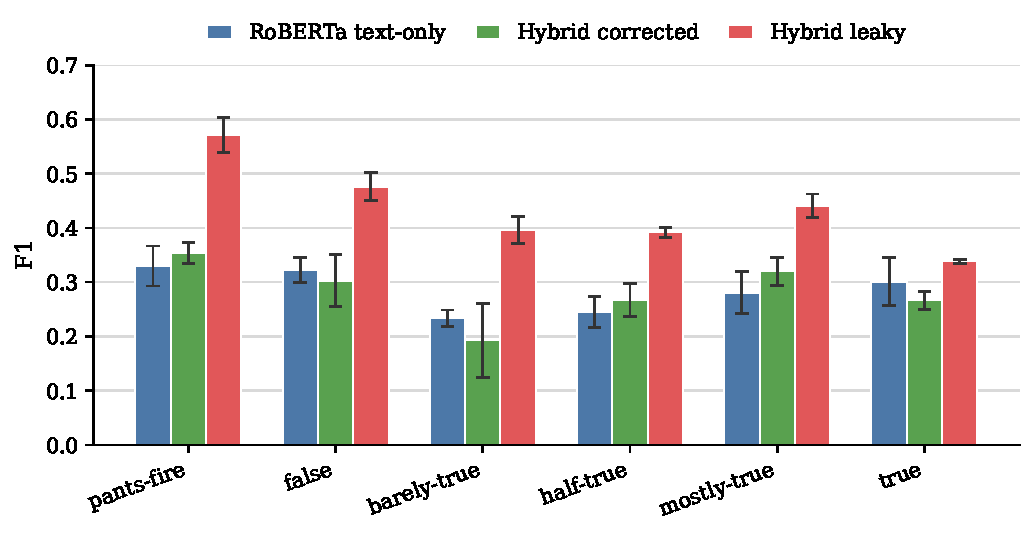
\includegraphics[width=0.95\textwidth]{figures/per_class_f1_grouped.pdf}
\caption{Seed-averaged per-class test F1 across seeds 42, 1337, and 2024. Bars show the mean and error bars show the across-seed standard deviation. The text-only RoBERTa and leakage-corrected hybrid have overlapping profiles, while the leaky hybrid lifts every class, with the largest gains concentrated on \emph{pants-fire}, \emph{false}, and \emph{mostly-true} where the credibility-history leakage is most diagnostic.}
\label{fig:perclass}
\end{figure*}

Two patterns are visible. First, the leakage-corrected hybrid does not dominate the text-only RoBERTa baseline class by class: the corrected hybrid is better on \emph{barely-true} ($+0.055$), \emph{mostly-true} ($+0.054$), and \emph{pants-fire} ($+0.015$), but worse on \emph{false} ($-0.056$), \emph{half-true} ($-0.025$), and \emph{true} ($-0.026$), netting to the $\pm$0 macro-F1 result reported above. The pattern is consistent with the known sensitivity of small-dataset transformer fine-tuning to seed and decoding noise rather than with a systematic metadata effect. Second, the per-class signature that has been used in the LIAR literature as evidence that metadata fusion encodes speaker reputation---large lifts on \emph{pants-fire} ($+0.283$ here) and \emph{mostly-true} ($+0.165$)---is observed only in the leaky regime. The same architecture, fed leakage-corrected credibility-history vectors, lifts \emph{pants-fire} by only $+0.015$ over the text-only baseline. We conclude that the per-class evidence for metadata fusion on LIAR is also leakage-driven.

\subsection{Leaky vs.\ Corrected: Quantifying the Leakage Signal}
Fig.~\ref{fig:cm_leaky_vs_corrected} compares the seed-averaged row-normalised confusion matrices of the leaky hybrid and the leakage-corrected hybrid on the test set. The diagonal mass of the leaky hybrid is dominant for every class---\emph{pants-fire} 57\%, \emph{false} 44\%, \emph{barely-true} 35\%, \emph{half-true} 37\%, \emph{mostly-true} 46\%, \emph{true} 41\%---and the off-diagonal mass is concentrated near the diagonal in an ordinal pattern. The leakage-corrected hybrid retains a much weaker diagonal across all classes and exhibits the same band of structured ordinal confusion that the text-only RoBERTa classifier produces. The qualitative reading is consistent with the quantitative one: removing the credibility-history leakage takes the model back to a regime in which the statement text alone is the primary signal.

\begin{figure*}[t]
\centering
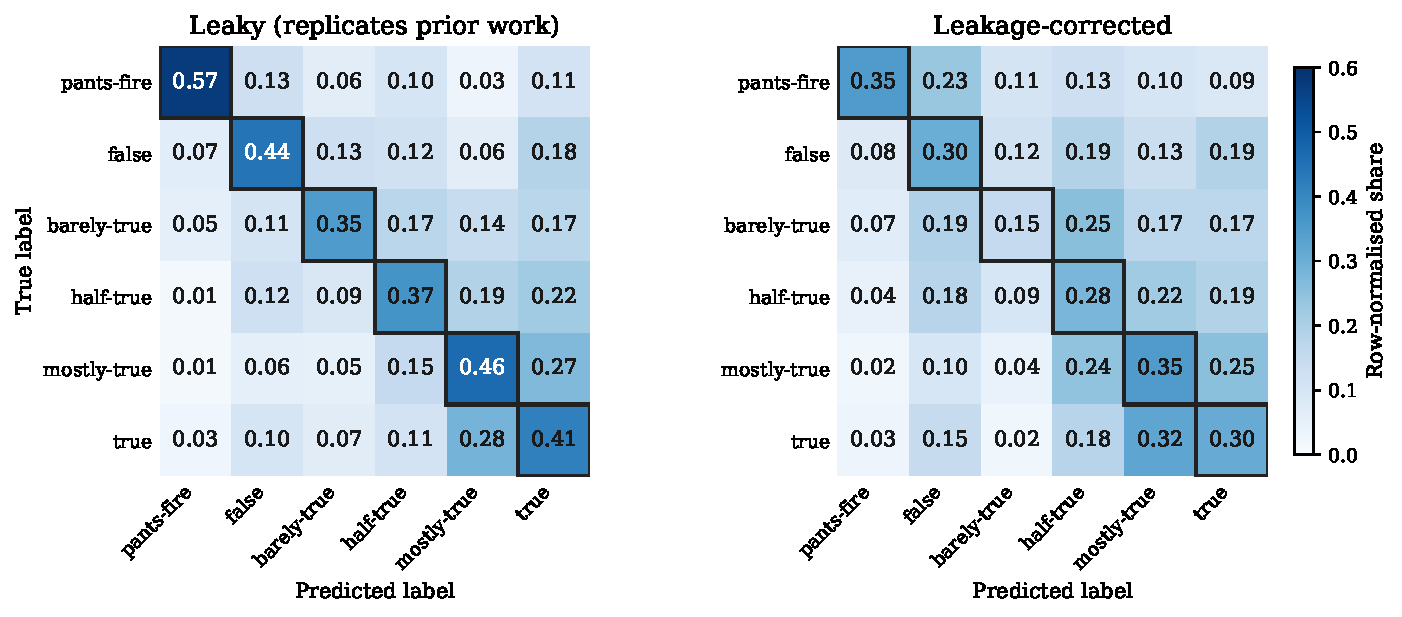
\includegraphics[width=0.95\textwidth]{figures/confusion_matrices.pdf}
\caption{Seed-averaged row-normalised confusion matrices on the LIAR test set across seeds 42, 1337, and 2024. Left: leaky hybrid, matching the prior LIAR metadata-fusion recipe. Right: leakage-corrected hybrid. The diagonal of the leaky model is uniformly stronger than the corrected model on every class; off-diagonal mass remains structured along the ordinal axis in both cases, but the corrected model resembles the text-only baseline in its overall confusion pattern.}
\label{fig:cm_leaky_vs_corrected}
\end{figure*}

\subsection{Metadata-Channel Ablation}
A complementary methodological concern is whether the leakage-corrected hybrid, although matched to the text-only RoBERTa on overall macro-F1, derives any incremental signal from the categorical metadata fields (\emph{speaker}, \emph{party}, \emph{job}, \emph{state}, \emph{subject}, \emph{context}) beyond the leaky credibility-history numbers. To address this we trained the same fusion architecture with both metadata branches masked (\emph{hybrid-textonly}). Across three seeds, the metadata-masked variant attains $0.287 \pm 0.009$ macro-F1, which is marginally above and statistically indistinguishable from the leakage-corrected hybrid ($0.284 \pm 0.003$) and the text-only RoBERTa ($0.285 \pm 0.007$). In other words, once the credibility-history leakage is removed, the categorical metadata branch on its own does not lift performance above the text-only baseline either. This is a stronger statement than ``the leakage explains the gain''; it is closer to ``the metadata channel does not provide measurable signal in the absence of leakage on LIAR.''

\subsection{Training Dynamics}
Fig.~\ref{fig:curves} plots training loss and validation macro-F1 across epochs for the four transformer-based systems on a representative training run. Two qualitative observations stand out. First, the leaky hybrid's validation macro-F1 separates early from the text-only RoBERTa, hybrid-textonly ablation, and leakage-corrected hybrid curves. The gap is established within the first few epochs of training and is reproducible across the three seeds. Second, the leakage-corrected hybrid's training and validation curves track the text-only and hybrid-textonly curves closely throughout training, which further confirms that the metadata branch on corrected inputs contributes no measurable signal beyond the text encoder.

\begin{figure*}[t]
\centering
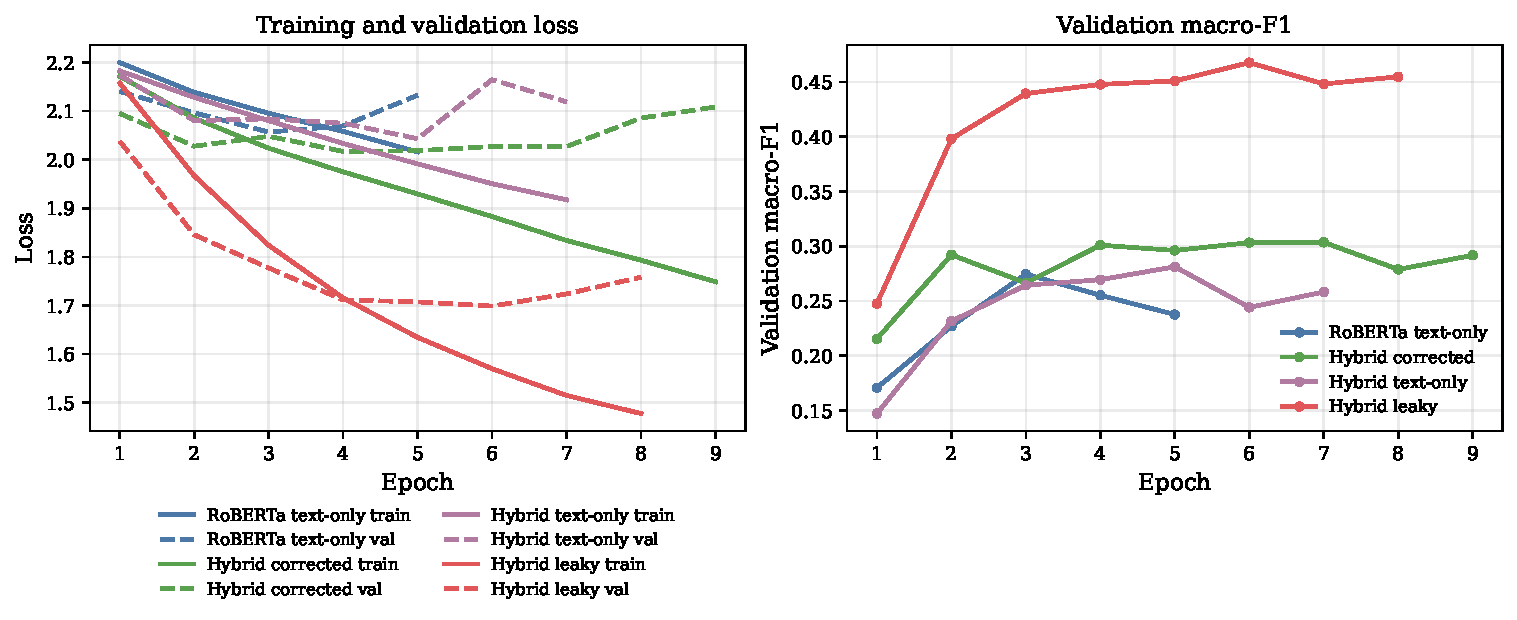
\includegraphics[width=0.95\textwidth]{figures/training_curves.pdf}
\caption{Training loss (left; solid curves = training loss, dashed curves = validation loss per model) and validation macro-F1 (right) for a representative training run. The leaky hybrid separates early from the other three transformer-based systems, while the text-only RoBERTa, leakage-corrected hybrid, and hybrid-textonly ablation track each other closely.}
\label{fig:curves}
\end{figure*}

% ======================================================================
\section{Discussion}
\label{sec:discussion}
% ======================================================================

\subsection{What Did the Apparent Metadata Gain Actually Buy?}
The headline of the previous section---a $+0.151$ macro-F1 gap between the leaky and the leakage-corrected hybrids on otherwise-identical architectures---admits a simple interpretation. The five-number credibility history is, under the released LIAR schema, an instance-level feature that contains the rating of the current statement itself. A hybrid classifier conditioned on this feature can therefore perform a fraction of the classification by reading off the leaked label, and this is exactly what we observe: the leaky hybrid concentrates its largest lifts on the classes where any single contribution is most diagnostic against a low base rate (\emph{pants-fire}) or against a class boundary that is hard to recover from text alone (\emph{mostly-true}/\emph{true}). Per-class analysis localises the leakage signal precisely where it should be expected if the leaky vector were doing the work; once the leakage is removed, the per-class gain disappears.

A complementary information-theoretic view is that the text of a 17-token political statement, by itself, carries a limited amount of information about its truthfulness, because political speech is rhetorically polished and rarely self-refuting. The leaky credibility-history vector is, formally, a noisy observation of the target label combined with prior counts, and that noisy observation alone is enough to explain the headline LIAR numbers reported in the literature. The categorical metadata (speaker, party, job, state, subject, context), in contrast, does not provide measurable lift in our experiments once the leakage is held out: the hybrid-textonly ablation attains essentially the same macro-F1 as the leakage-corrected hybrid.

\subsection{Relation to Published Results}
Our 0.436 macro-F1 in the leaky regime is consistent with the band of 0.41--0.44 macro-F1 reported by Long \emph{et~al.}~\cite{long2017fakenews}, by graph-attention systems~\cite{zhang2024heterosgt,gu2024,tong2025,zhang2024phd}, and by other LIAR hybrids that condition on the released credibility-history vector. We replicate this band cleanly: the leaky hybrid reaches $0.436 \pm 0.004$ macro-F1 across three seeds with a very simple concatenation fusion head on top of \texttt{roberta-base}, with no graph machinery and no per-class tuning. The fact that a deliberately simple architecture matches the published numbers is in itself diagnostic: the dominant signal in the leaky regime is the leakage, not the architecture.

The text-only RoBERTa baseline ($0.285$ macro-F1) and the leakage-corrected hybrid ($0.284$) place the no-leakage LIAR ceiling within a few points of the original 0.274 accuracy reported by Wang~\cite{wang2017liar}. This contradicts the popular narrative that \texttt{roberta-base} closes a large fraction of the LIAR gap on its own; a more accurate summary is that \texttt{roberta-base} closes a small fraction of the gap, that fraction is roughly the same as what the categorical metadata buys (i.e., none), and the remainder of the gap reported in prior work is attributable to credibility-history leakage. We therefore recommend that future LIAR studies report results in both the leaky and the leakage-corrected regimes, treating the gap between the two as an artifact of the dataset rather than as a property of the model.

\subsection{Implications for the LIAR Literature}
Three implications follow. First, the comparison between LIAR and other fact-checking benchmarks should be re-examined in the leakage-corrected regime: the cross-benchmark generalisation gap reported by Ma \emph{et~al.}~\cite{ma2024emnlp} and Villela \emph{et~al.}~\cite{villela2023} is partly a comparison between an in-distribution leakage-augmented baseline and an out-of-distribution clean baseline, which over-estimates the true generalisation gap. Second, the apparent advantage of graph-based and attention-based hybrids over flat fusion on LIAR is plausibly driven by their being slightly better at exploiting the same leakage signal, rather than by their architectural sophistication; a fair comparison would require running each architecture in both regimes. Third, future LIAR-derived benchmarks should compute credibility-history features in a leave-one-out manner at construction time, so that any model trained on them is structurally prevented from accessing the current label.

\subsection{Limitations}
Several limitations of this work should be stated explicitly. Our leakage correction assumes that the released credibility-history columns include exactly one contribution from the current statement. We verify this empirically across all three released splits (Section III-C) but did not re-scrape PolitiFact to confirm the counting convention for every individual speaker. First, LIAR is an in-distribution benchmark: all of train, validation, and test come from the same PolitiFact pipeline. Our leakage-correction procedure is formally exact under the assumption that the released credibility-history columns count exactly the speaker's PolitiFact ratings up to and including the current statement; if a different counting convention is used in any sub-corpus, the corrected vector will inherit a residual bias whose magnitude we cannot quantify without re-scraping PolitiFact. Second, although we report three independent seeds for every transformer-based system, the variance band on small datasets remains broad enough that 5--10 seeds would yield tighter confidence intervals; we flag this as a follow-up. Third, the fusion head we use is a flat concatenation with a small MLP, and we have not re-run more sophisticated fusion mechanisms (cross-attention, gating by speaker-reliability, graph-based designs~\cite{zhang2024heterosgt}) in the leakage-corrected regime. Doing so is left for future work and is, in our view, the most informative next experiment for the LIAR literature. Fourth, the categorical metadata is hashed rather than embedded from the vocabulary; this removes a vocabulary-mismatch failure mode at inference time but sacrifices a small amount of representational capacity at training time.

\subsection{Ethical and Deployment Considerations}
A disinformation-detection system that relies heavily on speaker identity could, if deployed naively, systematically disadvantage speakers whose metadata profiles happen to resemble historical fabricators. The result we report here---that this reliance does not actually buy measurable accuracy on LIAR once leakage is removed---is therefore relevant beyond the methodological audit: it argues against deploying credibility-history-conditioned classifiers in production settings on the basis of their LIAR numbers alone. We recommend that practitioners who adapt the hybrid architecture to other datasets (i)~report per-subgroup F1 rather than only overall macro-F1, (ii)~disable the credibility-history channel for first-time speakers, (iii)~compute credibility-history-style features in a leave-one-out manner over the production corpus, and (iv)~compare against a text-only baseline as a sanity check.

% ======================================================================
\section{Conclusion and Future Work}
\label{sec:conclusion}
% ======================================================================
We revisited the LIAR six-class disinformation benchmark and asked a deliberately narrow question: how much of the previously-reported metadata-fusion gain over text-only baselines is attributable to label leakage in the credibility-history features released with the dataset? Our answer is concrete and measurable: across three seeds, the leaky hybrid attains $0.436 \pm 0.004$ macro-F1 on the canonical LIAR test split, reproducing the published band of metadata-fusion numbers on this benchmark. The leakage-corrected hybrid drops to $0.284 \pm 0.003$ macro-F1, statistically indistinguishable from a text-only RoBERTa baseline ($0.285 \pm 0.007$) and from a matched architectural ablation that masks the metadata branch entirely ($0.287 \pm 0.009$). The per-class signature historically used as evidence that metadata fusion encodes speaker reputation---large lifts on \emph{pants-fire} and \emph{mostly-true}---is observed only in the leaky regime and disappears once leakage is corrected.

Three directions define our planned future work. First, a wider multi-seed evaluation (5--10 seeds per system) and seed-stratified bootstrap confidence intervals will tighten the bands on the headline numbers and quantify the known seed sensitivity of small-dataset transformer fine-tuning. Second, a matched out-of-distribution evaluation on FakeNewsNet~\cite{shu2017} and ISOT~\cite{sadeghi2022} in both the leaky and the leakage-corrected regimes will probe whether the LIAR-internal leakage finding generalises to other fact-checking corpora that ship with similar speaker-reputation features. Third, we intend to re-run the leading graph- and attention-based LIAR hybrids~\cite{zhang2024heterosgt,gu2024,tong2025,zhang2024phd} under our leakage-corrected preprocessing and report a side-by-side leaderboard, which we believe is the most useful single follow-up that this paper invites. The full codebase, multi-seed metric JSONs, per-example prediction artifacts, and a Boolean configuration flag that toggles the leakage correction are public at \url{https://github.com/nihsioK/nlp-disinformation-detection-aitu}, and we hope the leaky-vs-corrected reporting protocol introduced here will be reused by subsequent work on this benchmark.

% % ======================================================================
% \section*{Acknowledgements}
% % ======================================================================
% The author thanks Prof.~Tamara Zhukabayeva for supervision throughout the MSc programme, and the Astana IT University Department of Computer Science and Engineering for hardware access during the pipeline-development phase. All training reported in this paper was run on publicly available Kaggle compute.

% ======================================================================
% References
% ======================================================================
\bibliographystyle{IEEEtran}
\bibliography{references}

\end{document}
